\section{Tìm hiểu về đa kế thừa trong C++.}

\subsection{Khái niệm về đa kế thừa.}
Ngôn ngữ C++ cho phép một lớp kế thừa từ nhiều lớp cơ sở cùng lúc.
Đây được gọi là kế thừa đa lớp (hay đa kế thừa), giúp kết hợp các tính năng từ các hệ thống phân cấp lớp khác nhau.

-- \textbf{Cú pháp:}
\lstinputlisting{code/Cau01_Code01.cpp}

-- \textbf{Ví dụ minh họa:}
\lstinputlisting{code/Cau01_Code02.cpp}

-- \textbf{Giải thích:}
\begin{itemize}
    \item[$+$] Lớp MultiFunctionDevice bây giờ có thể truy cập các phương thức từ cả lớp Printer và lớp Scanner.
    \item[$+$] Các hàm khởi tạo được gọi theo thứ tự các lớp cơ sở xuất hiện trong khai báo kế thừa,
               từ trái sang phải. Các hàm hủy được gọi theo thứ tự ngược lại.
               Có thể truyền đối số cho từng hàm khởi tạo của lớp cơ sở trong danh sách khởi tạo.
\end{itemize}

\subsection{Vấn đề trùng tên hàm trong đa kế thừa.}
Có trường hợp hai lớp cơ sở có các hàm trùng tên với nhau, các hàm này không được định nghĩa lại trong lớp dẫn xuất.
Nếu đối tượng của lớp dẫn xuất gọi các hàm đó thì trình biên dịch sẽ báo lỗi vì nó không biết là đối tượng của lớp dẫn xuất
muốn gọi hàm trong lớp cơ sở nào.

-- \textbf{Ví dụ minh họa:}
\lstinputlisting{code/Cau01_Code03.cpp}

-- \textbf{Giải thích:} Ở dòng 37, nếu ta xóa comment (“//”) trước lệnh “object.input();” thì trình biên dịch 
sẽ báo lỗi là: “DerivedClass::input” is ambiguous. Để giải quyết vấn đề này, ta phải chỉ rõ là ta đang gọi hàm input() 
của lớp cơ sở nào (BaseClass01 hay BaseClass02), bằng cách sử dụng toán tử phân giải phạm vi “::”.

-- \textbf{Giải pháp:} Sử dụng toán tử phân giải phạm vi “::”.
\lstinputlisting{code/Cau01_Code04.cpp}

\subsection{Vấn đề trùng tên thuộc tính trong đa kế thừa.}
Hiện tượng trùng tên thuộc tính trong đa kế thừa là hiện tượng phát sinh khi một lớp dẫn xuất kế thừa 
đồng thời từ nhiều lớp cơ sở có khai báo các thành viên dữ liệu trùng tên thuộc tính, 
dẫn đến sự mơ hồ trong phân giải tên tại thời điểm biên dịch hoặc vận hành. 
Đồng thời, nó có nguy cơ gây ra sự dư thừa trạng thái thông qua việc nhân bản nhiều thực thể của cùng một thuộc tính.

-- \textbf{Ví dụ minh họa:} Lớp C kế thừa từ cả hai lớp A và B đều có thuộc tính x.
\lstinputlisting{code/Cau01_Code05.cpp}

-- \textbf{Giải thích:} Ở dòng 23, nếu ta xóa comment (“//”) trước lệnh “cout << object.x;” thì trình biên dịch sẽ 
báo lỗi là: “C::x” is ambiguous. Để giải quyết vấn đề này, ta có thể sử dụng toán tử phân giải phạm vi “::” để 
chỉ rõ là ta muốn truy cập thuộc tính x của lớp nào (lớp A hay lớp B), hoặc ta cũng có thể sử dụng từ khóa “using” 
bên trong lớp C nếu ta muốn mặc định lớp C chỉ sử dụng thuộc tính x của một lớp cơ sở nhất định (hoặc của lớp A, hoặc của lớp B).

-- \textbf{Giải pháp 01:} Sử dụng toán tử phân giải phạm vi “::”.
\lstinputlisting{code/Cau01_Code06.cpp}

-- \textbf{Giải pháp 02:} Sử dụng từ khóa “using”.
\lstinputlisting{code/Cau01_Code07.cpp}

\subsection{Vấn đề hình thoi trong đa kế thừa.}
Vấn đề hình thoi trong đa kế thừa xảy ra khi một lớp dẫn xuất kế thừa từ hai lớp cơ sở, 
mà bản thân hai lớp cơ sở đó lại kế thừa từ một lớp cơ sở khác. Điều này gây ra sự mơ hồ vì lớp dẫn xuất cuối cùng 
có nhiều bản sao của cùng một thành viên của lớp cơ sở, khiến việc truy cập thành viên trở nên không rõ ràng. 
Nói một cách đơn giản, lớp con kế thừa từ hai lớp cha, mà cả hai lớp cha đều đã kế thừa từ cùng một lớp cơ sở.
Như vậy, lớp con nhận được hai bản sao của cùng một lớp cơ sở, gây ra sự mơ hồ.

\begin{center}
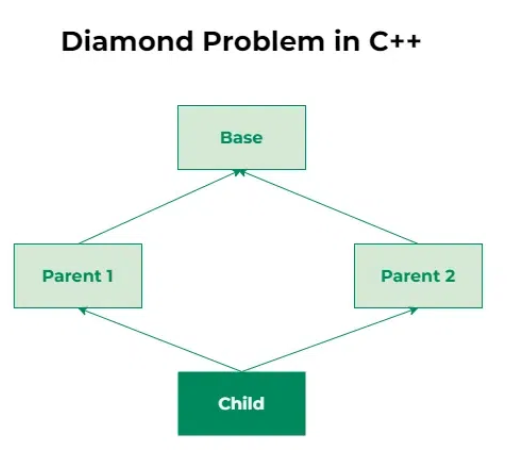
\includegraphics[width=0.5\textwidth]{images/DiamondProblem.png}
\end{center}

-- \textbf{Ví dụ minh họa:}
\lstinputlisting{code/Cau01_Code08.cpp}

-- \textbf{Giải thích:} Ở dòng 25, nếu ta xóa comment (“//”) trước lệnh “object.fun();” thì trình biên dịch sẽ 
báo lỗi là: “Child::fun” is ambiguous. Điều này bắt nguồn từ các lý do sau: lớp Base định nghĩa hàm fun(), 
cả hai lớp Parent01 và Parent02 đều kế thừa từ lớp Base; lớp Child kế thừa từ cả hai lớp Parent01 và Parent02, 
dẫn đến việc có hai bản sao của lớp Base. Lệnh “object.fun();” không rõ ràng vì trình biên dịch không thể quyết định 
nên gọi hàm Base::fun() nào.

-- \textbf{Giải pháp:} Ngôn ngữ C++ giải quyết vấn đề hình thoi bằng cách sử dụng “kế thừa ảo” (virtual inheritance). 
Kế thừa ảo đảm bảo rằng chỉ có một thể hiện chung duy nhất của lớp cơ sở tồn tại, bất kể nó được kế thừa bao nhiêu lần.
\lstinputlisting{code/Cau01_Code09.cpp}

-- \textbf{Giải thích:} Ta đã sử dụng từ khóa “virtual” khi hai lớp Parent01 và Parent02 kế thừa lớp Base (lần lượt ở dòng 10 và dòng 14), 
giúp hợp nhất vùng nhớ của lớp Base. Khi đó, lớp Child kế thừa đồng thời từ hai lớp Parent01 và Parent02 chỉ có một bản sao của lớp Base, 
lệnh “object.fun();” được giải quyết một cách rõ ràng.